\chapter{Ordenación avanzada}
En este caso se presentan algoritmos de ordenación más eficientes que los vistos en el capítulo anterior. Estos algoritmos son más eficientes en términos de tiempo de ejecución y se basan en la técnica de dividir y conquistar. Podría verse mas como una ordenación de ficheros.

\begin{figure}[h]
\centering
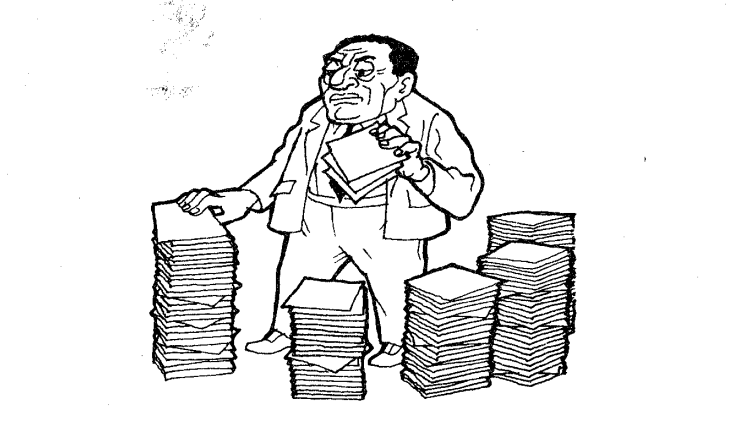
\includegraphics[scale=0.9]{./estáticos/ordenacionFicheros.png}
\caption{Ordenación de ficheros}
\end{figure}

\section{Ordenación por mezcla (Merge Sort)}
El algoritmo de ordenación por mezcla es un algoritmo recursivo que se basa en la técnica de dividir y conquistar. Este algoritmo consiste en dividir el arreglo a ordenar en varias partes, estas partes se ordenan y, posteriormente, se mezclan entre ellas de forma ordenada. Dado que el proceso de mezcla es menos costoso que el proceso de ordenación obtenemos un algoritmo más eficiente.

El algoritmo de ordenación por mezcla se basa en los siguientes principios:
\begin{enumerate}
    \item Dividir recursivamente el arreglo en 2 partes.
    \item Si el arreglo tiene un solo elemento, entonces está ordenado por definición.
    \item Si la lista tiene más de un ítem, dividimos la lista e invocamos recursivamente un ordenamiento por mezcla para ambas mitades.
    \item Una vez que ambas mitades estén ordenadas, la operación de mezcla se encarga de unir ambas mitades en un solo arreglo ordenado.
\end{enumerate}

El proceso de división puede verse de la siguiente manera:

\newpage
\begin{figure}[h]
\centering
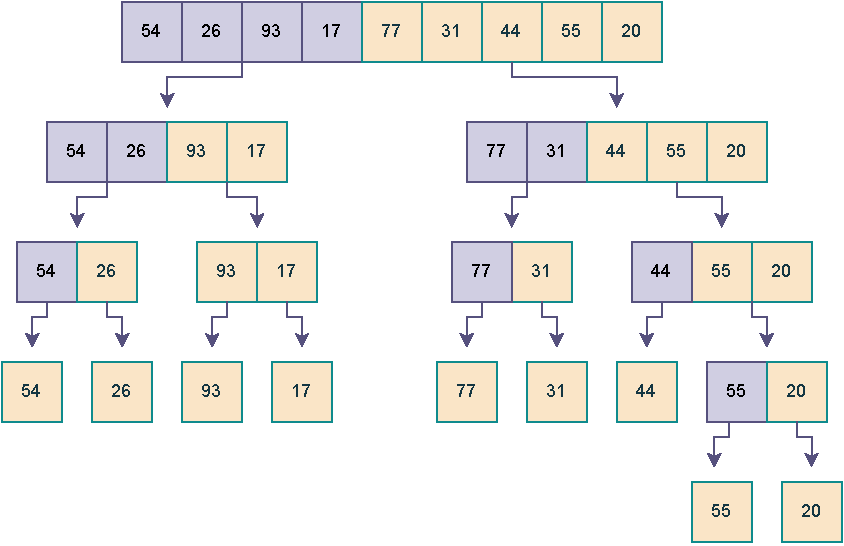
\includegraphics[scale=0.88]{./estáticos/mergediv.pdf}
\caption{Ejemplo de proceso de división}
\end{figure}

El proceso de mezcla puede verse de la siguiente manera:

\begin{figure}[h]
\centering
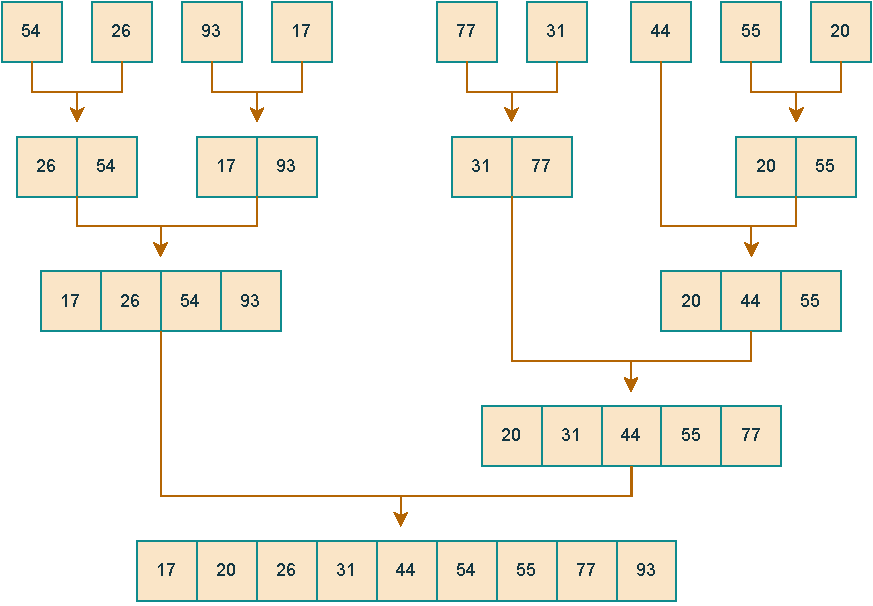
\includegraphics[scale=0.88]{./estáticos/mergemezcla.pdf}
\caption{Ejemplo de proceso de mezcla}
\end{figure}

\subsection{Idea de crear el código}
La idea es definir un procedimiento al que le pasamos en qué parte del arreglo queremos hacer lo fundamental del mergesort: dividirlo en dos, ordenar cada mitad y luego intercalar las dos mitades. Este procedimiento es \texttt{merge\_sort\_rec}, que toma el arreglo a y las posiciones inicial y final del pedazo de arreglo que vamos a ordenar. El procedimiento principal llama al recursivo con los índices 1 y n (el arreglo completo).

\begin{codebox}{Código 26}
\footnotesize Estructura de la función merge\_sort
\tcblower
\begin{pascallike}
proc merge_sort(in/out a: array[1..n] of T)
    merge_sort_rec(a,1,n)
end proc
proc merg_sort_rec(in/out a: array[1..n] of T, in lft,rgt: nat)
...
end proc
\end{pascallike}
\end{codebox}

El procedimiento \texttt{merge\_sort\_rec} toma el arreglo a, y los índices \textbf{lft} y \textbf{rgt}, que corresponden con el comienzo y el final del pedazo de arreglo que queremos ordenar. Recordando la idea del algoritmo, el caso más simple es cuando el pedazo de arreglo tiene un solo elemento. En nuestra implementación eso corresponde a que lft sea igual a rgt. En ese caso el procedimiento no debe hacer nada, ya que el pedazo está trivialmente ordenado.
En caso que no se dé esa situación, debemos:
\begin{enumerate}
    \item Dividir el pedazo de arreglo en dos,
    \item ordenar cada una de esas mitades utilizando el mismo algoritmo, e
    \item intercalar cada mitad ordenada.
\end{enumerate}
Para dividir el pedazo de arreglo, se define una variable \textbf{mid} de tipo nat a la que se le asigna el índice correspondiente a la posición del medio.

\begin{codebox}{Código 27}
\footnotesize División del arreglo
\tcblower
\begin{pascallike}
proc merg_sort_rec(in/out a: array[1..n] of T, in lft,rgt: nat)
    var mid: nat
    if rgt > lft --> mid := (rgt+lft) `div` 2
    ...
end proc
\end{pascallike}
\end{codebox}
Ahora entonces hay que llamar recursivamente al procedmiento dos veces: una para la primera mitad que irá desde la posición \textbf{lft} hasta \textbf{mid}, y otra para la segunda mitad, que irá desde la posición \textbf{mid+1} hasta \textbf{rgt}.
\begin{codebox}{Código 28}
\footnotesize Llamada recursiva
\tcblower
\begin{pascallike}
proc merg_sort_rec(in/out a: array[1..n] of T, in lft,rgt: nat)
    var mid: nat
    if rgt > lft --> mid := (rgt+lft) `div` 2
    merge_sort_rec(a,lft,mid)
    merge_sort_rec(a,mid+1,rgt)
    ...
end proc
\end{pascallike}
\end{codebox}
y por último, hay que intercalar. Esta tarea la implementaremos con un procedimiento llamado \texttt{merge}, que se define mas adelante.
\begin{codebox}{Código 29}
\footnotesize Definición completa de la función merge\_sort\_rec
\tcblower
\begin{pascallike}
proc merg_sort_rec(in/out a: array[1..n] of T, in lft,rgt: nat)
    var mid: nat
    if rgt > lft --> mid := (rgt+lft) `div` 2
    merge_sort_rec(a,lft,mid)
    merge_sort_rec(a,mid+1,rgt)
    merge(a,lft,mid,rgt)
end proc
\end{pascallike}
\end{codebox}
Ahora para implementar el procedimiento de \textbf{intercalación}, se necesita un arreglo auxiliar, en donde se van a guardar los valores de la primera mitad a intercalar.
Se define entonces una variable de tipo array, dos variables en las que luego almacenaremos índices \texttt{j} y \texttt{k}, y se copia la primera mitad del arreglo en el arreglo auxiliar:
\begin{codebox}{Código 30}
\footnotesize Inicialización de variables
\tcblower
\begin{pascallike}
proc merge(in/out a: array[1..n] of T, in lft,mid,rgt: nat)
    var tmp: array[1..n] of T
    var j,k: nat
    for i:=lft to mid do ->
        tmp[i] := a[i] 
    od
    ...
end proc
\end{pascallike}
\end{codebox}
Los índices \texttt{j} y \texttt{k} indicarán respectivamente el elemento de la primera mitad que estoy analizando para insertar en el pedazo de arreglo que quedará ordenado, y el índice de la segunda mitad que estoy analizando. Inicialmente observo el primero de cada mitad, es decir \textbf{lft} y \textbf{mid+1}.
\begin{codebox}{Código 31}
\footnotesize Inicialización de índices
\tcblower
\begin{pascallike}
proc merge(in/out a: array[1..n] of T, in lft,mid,rgt: nat)
    var tmp: array[1..n] of T
    var j,k: nat
    for i:=lft to mid do ->
        tmp[i] := a[i] 
    od
    j := lft
    k := mid+1
    ...
end proc
\end{pascallike}
\end{codebox}
Ahora hay que rellenar el pedazo completo de arreglo que contendrá las dos mitades intercaladas ordenadamente. Lo recorro con un for desde lft hasta rgt. Y se puede ver que en cada paso si el elemento que estoy observando de la primera mitad es menor o igual que el de la segunda mitad, de acuerdo a esa comparación sabré qué elemento va a ubicarse en el arreglo ordenado.
\begin{codebox}{Código 32}
\footnotesize Intercalación
\tcblower
\begin{pascallike}
proc merge(in/out a: array[1..n] of T, in lft,mid,rgt: nat)
    var tmp: array[1..n] of T
    var j,k: nat
    for i:=lft to mid do ->
        tmp[i] := a[i] 
    od
    j := lft
    k := mid+1
    for i:=lft to rgt do ->
        if j <= mid && (k > rgt || tmp[j] <= a[k])
            then a[i] := tmp[j]
                j:= j+1
            else a[i] := a[k]
                k := k+1
        fi
    od
end proc
\end{pascallike}
\end{codebox}
En la guarda del if hay que considerar también el caso en que ya haya agotado todos los elementos de la segunda mitad, lo que sucederá cuando \texttt{k > rgt}, y entonces en ese caso también completo con los elementos de la primera mitad (es decir los que están en el arreglo auxiliar).

\subsection{Análisis de complejidad}
Para analizar la función, debemos considerar los dos procesos distintos que conforman su implementación. En primer lugar, la lista se divide en mitades. Podemos dividir una lista por la mitad en un tiempo $\log n$ donde $n$ es la longitud de la lista. El segundo proceso es la mezcla. Cada ítem de la lista se procesará y se colocará en la lista ordenada. Así que la operación de mezcla que da lugar a una lista de tamaño n requiere n operaciones. El resultado de este análisis es que se hacen $\log n$ divisiones, cada una de las cuales cuesta $n$ para un total de $n\log n$ operaciones. Un ordenamiento por mezcla es un algoritmo $O(n \log n)$.

\subsection{Código}

\begin{codebox}{Código 33}
\footnotesize Ordenación por mezcla (Merge Sort)
\tcblower
\begin{pascallike}
proc merge_sort(in/out a: array[1..n] of T)
    merge_sort_rec(a,1,n)
end proc

proc merge_sort_rec(in/out a: array[1..n] of T, in lft,rgt: nat)
    var mid: nat
    if rgt > lft --> mid := (rgt+lft) `div` 2
        merge_sort_rec(a,lft,mid)
        merge_sort_rec(a,mid+1,rgt)
        merge(a,lft,mid,rgt)
    fi
end proc

proc merge(in/out a: array[1..n] of T, in lft,mid,rgt: nat)
    var tmp: array[1..n] of T
    var j,k: nat
    for i:=lft to mid do ->
        tmp[i] := a[i] 
    od
    j := lft
    k := mid+1
    for i:=lft to rgt do ->
        if j <= mid && (k > rgt || tmp[j] <= a[k])
            then a[i] := tmp[j]
                j:= j+1
            else a[i] := a[k]
                k := k+1
        fi
    od
end proc
\end{pascallike}
\end{codebox}

\section{Ordenación rápida (Quick Sort)}
El ordenamiento rápido usa dividir y conquistar para obtener las mismas ventajas que el ordenamiento por mezcla, pero sin utilizar almacenamiento adicional. Sin embargo, es posible que la lista no se divida por la mitad. Cuando esto sucede, el desempeño disminuye.

El algoritmo de ordenación rápida se basa en los siguientes principios:
\begin{enumerate}
    \item Primero selecciona un valor, que se denomina el \textbf{pivot} (El papel del valor pivote es ayudar a dividir la lista).
    \item La posición real a la que pertenece el valor pivote en la lista final ordenada, comúnmente denominado punto de división, se utilizará para dividir la lista para las llamadas posteriores a la función de ordenamiento rápido.
    \item El proceso de partición sucederá a continuación. Encontrará el punto de división y al mismo tiempo moverá otros ítems al lado apropiado de la lista, según sean menores o mayores que el valor pivote.
\end{enumerate}

A modo ilustrativo, se puede ver el proceso de partición en la siguiente figura:

\begin{figure}[h]
\centering
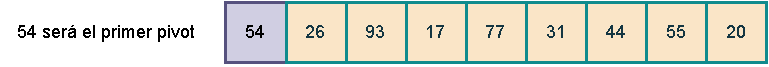
\includegraphics[scale=0.88]{./estáticos/pivot.pdf}
\caption{Ejemplo de proceso de partición}
\end{figure}

El particionamiento comienza localizando dos marcadores de posición \texttt{lft} y \texttt{rgt} al principio y al final de los ítems restantes de la lista. El objetivo del proceso de partición es mover ítems que están en el lado equivocado con respecto al valor pivote mientras que también se converge en el punto de división.

\begin{figure}[h]
\centering
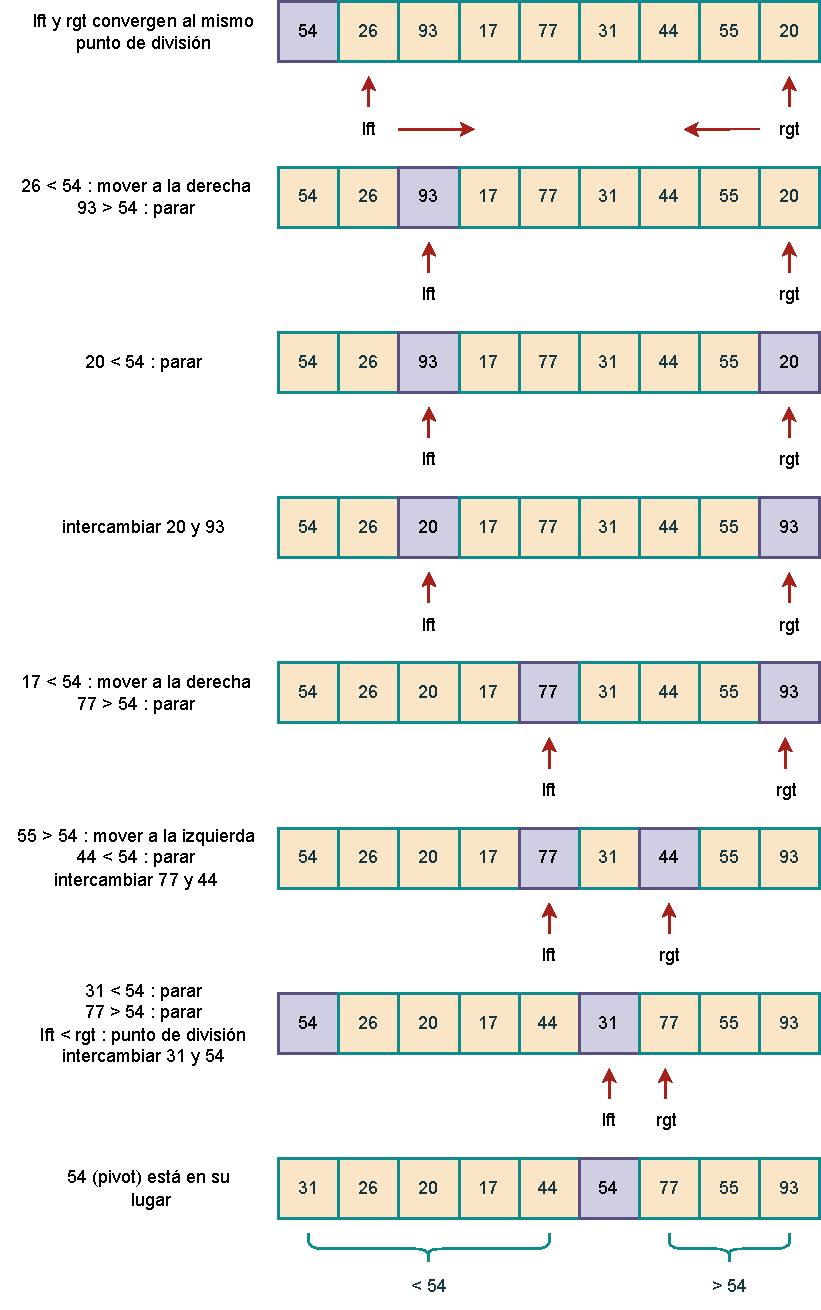
\includegraphics[scale=0.74]{./estáticos/quick.pdf}
\caption{Ejemplo de proceso}
\end{figure}

\begin{itemize}
    \item Comienza incrementando \texttt{lft} hasta que localicemos un valor que sea mayor que el valor pivote. Luego decrementamos \texttt{rgt} hasta que encontremos un valor que sea menor que el valor pivote. En tal punto habremos descubierto dos ítems que están fuera de lugar con respecto al eventual punto de división. 
    \item Para este ejemplo, esto ocurre en 93 y 20. Ahora se deben intercambiar estos dos ítems y luego repetir el proceso de nuevo.
    \item Se detiene en el punto donde \texttt{rgt} se vuelva menor que \texttt{lft}. La posición de \texttt{lft} es ahora el punto de división. El valor pivote se puede intercambiar con el contenido del punto de división y el valor pivote está ahora en su lugar.
\end{itemize}
\textit{ La lista ahora se puede dividir en el punto de división y el ordenamiento rápido se puede invocar recursivamente para las dos mitades.}

\subsection{Idea de crear el código}
De manera similar al algoritmo de ordenación \texttt{merge\_sort}, se define un procedimiento recursivo que tomará el arreglo de elementos y dos índices correspondientes al pedazo de arreglo que se ordenará. El algoritmo principal llama a este procedimiento con los índices \texttt{1} y \texttt{n}, correspondiendo con la ordenación del arreglo completo.

\begin{codebox}{Código 34}
\footnotesize Estructura de la función quick\_sort
\tcblower
\begin{pascallike}
proc quick_sort(in/out a: array[1..n] of T)
    quick_sort_rec(a,1,n)
end proc
proc quick_sort_rec(in/out a: array[1..n] of T, in lft,rgt: nat)
...
end proc
\end{pascallike}
\end{codebox}
Este procedimiento recursivo tiene su caso más simple cuando \textbf{lft} y \textbf{rgt} son iguales, lo que significa que estoy ordenando un arreglo de un solo elemento. En el caso interesante, al procedimiento se lo llama partition que será el encargado de acomodar los elementos del pedazo de arreglo utilizando el elemento de más a la izquierda como \textbf{pivot}.
\begin{codebox}{Código 35}
\footnotesize Llamada a la función partition
\tcblower
\begin{pascallike}
proc quick_sort_rec(in/out a: array[1..n] of T, in lft,rgt: nat)
    var ppiv: nat
    if rgt > lft --> 
        partition(a,lft,rgt,ppiv)
    ...
...
end proc
\end{pascallike}
\end{codebox}
El procedimiento \texttt{partition} modifica el arreglo desde \texttt{lft} hasta \texttt{rgt} dejando al comienzo todos los elementos que son menores o iguales al que se encontraba originalmente en la posición \texttt{lft}, y al final a todos los que son mayores o iguales. También modifica la variable \texttt{ppiv} asignándole el índice correspondiente al lugar donde queda ubicado definitivamente el elemento que se usó como \textbf{pivot}.
Luego lo único que queda por hacer es llamar recursivamente al procedimiento, una vez para los elementos que quedaron acomodados a la izquierda del pivot, y otra vez para los elementos que quedaron acomodados a la derecha.
\begin{codebox}{Código 36}
\footnotesize Llamada recursiva
\tcblower
\begin{pascallike}
proc quick_sort_rec(in/out a: array[1..n] of T, in lft,rgt: nat)
    var ppiv: nat
    if rgt > lft --> 
        partition(a,lft,rgt,ppiv)
        quick_sort_rec(a,lft,ppv-1)
        quick_sort_rec(a,ppiv+1,rgt)
    fi
end proc
\end{pascallike}
\end{codebox}
Queda por ver el procedimiento partition. Toma el arreglo, los dos índices que indican qué fragmento estamos ordenando, y una variable de solo escritura, en la cual indicaremos el índice en donde queda el pivot una vez que finalice el procedimiento.

\begin{codebox}{Código 37}
\footnotesize Estructura de la función partition
\tcblower
\begin{pascallike}
proc partition(in/out a: array[1..n] of T, in lft,rgt: nat, out ppiv: nat)
...
end proc
\end{pascallike}
\end{codebox}
Lo que hay que hacer en este procedimiento es ir mirando con un índice los elementos que están a la izquierda y con otro los que están a la derecha. El índice \texttt{i} indicará el elemento que estoy mirando desde la izquierda, y respectivamente \texttt{j} indicará el de la derecha. El elemento tomado como \textbf{pivot} será el que está más a la izquierda.
\begin{codebox}{Código 38}
\footnotesize Inicialización de variables
\tcblower
\begin{pascallike}
proc partition(in/out a: array[1..n] of T, in lft,rgt: nat, out ppiv: nat)
    var i,j: nat
    ppiv:= lft
    i:= lft+1
    j:= rgt
    ...
end proc
\end{pascallike}
\end{codebox}
Luego hay que ir viendo si el elemento indicado con el índice \texttt{i} y el indicado con \texttt{j} están bien ubicados, es decir, si \texttt{a[i]} es menor o igual al \textbf{pivot}, y si \texttt{a[j]} es mayor o igual. En caso que sea así, \texttt{"avanzo"} el índice. Este avance corresponde a sumar uno para \texttt{i}, y a restar uno para \texttt{j}. En caso que el elemento de la izquierda esté mal ubicado, debemos encontrar un elemento de la derecha que también esté mal ubicado, y los intercambiamos.
\begin{codebox}{Código 39}
\footnotesize Particionamiento
\tcblower
\begin{pascallike}
proc partition(in/out a: array[1..n] of T, in lft,rgt: nat, out ppiv: nat)
    var i,j: nat
    ppiv:= lft
    i:= lft+1
    j:= rgt
    do i <= j -->
        if a[i] <= a[ppiv] --> i:= i+1
            a[j] >= a[ppiv] --> j:= j-1
            a[i] > a[ppiv] && a[j] < a[ppiv] --> swap(a,i,j)
        fi
    od
...
end proc
\end{pascallike}
\end{codebox}
Esto se repite hasta que los índices \texttt{i} y \texttt{j} se hayan cruzado. En ese momento se termina el ciclo y solo queda ubicar correctamente al elemento \textbf{pivot}, y asignar la variable \texttt{ppiv} para que indique la posición final en donde queda el mismo.

\begin{codebox}{Código 40}
\footnotesize Finalización del procedimiento
\tcblower
\begin{pascallike}
proc partition(in/out a: array[1..n] of T, in lft,rgt: nat, out ppiv: nat)
    var i,j: nat
    ppiv:= lft
    i:= lft+1
    j:= rgt
    do i <= j --> if a[i] <= a[ppiv] --> i:= i+1
                        a[j] >= a[ppiv] --> j:= j-1
                        a[i] > a[ppiv] && a[j] < a[ppiv] --> swap(a,i,j)
                    fi
    od
    swap(a,ppiv,j)
    ppiv:= j
end proc
\end{pascallike}
\end{codebox}

\subsection{Análisis de complejidad}
Para analizar la función, hay que tener en cuenta que para una lista de longitud $n$, si la partición siempre ocurre en el centro de la lista, habrá de nuevo $\log n$ divisiones. Con el fin de encontrar el punto de división, cada uno de los $n$ ítems debe ser comparado contra el valor pivote. El resultado es $n\log n$ . Además, no hay necesidad de memoria adicional como en el proceso de ordenamiento por mezcla.
En el peor de los casos, los puntos de división pueden no estar en el centro y podrían estar muy sesgados a la izquierda o a la derecha, dejando una división muy desigual. En este caso, ordenar una lista de $n$ ítems se divide en ordenar una lista de $0$ ítems y una lista de $n-1$ ítems. Similarmente, ordenar una lista de tamaño $n-1$ se divide en una lista de tamaño $0$ y una lista de tamaño $n-2$ y así sucesivamente. El resultado es un ordenamiento $O(n^2)$ con toda la sobrecarga que requiere la recursión.

\subsection{Código}

\begin{codebox}{Código 41}
\footnotesize Ordenación rápida (Quick Sort)
\tcblower
\begin{pascallike}
proc quick_sort(in/out a: array[1..n] of T)
    quick_sort_rec(a,1,n)
end proc

proc quick_sort_rec(in/out a: array[1..n] of T, in lft,rgt: nat)
    var ppiv: nat
    if rgt > lft --> 
        partition(a,lft,rgt,ppiv)
        quick_sort_rec(a,lft,ppv-1)
        quick_sort_rec(a,ppiv+1,rgt)
    fi
end proc

proc partition(in/out a: array[1..n] of T, in lft,rgt: nat, out ppiv: nat)
    var i,j: nat
    ppiv:= lft
    i:= lft+1
    j:= rgt
    do i <= j --> if a[i] <= a[ppiv] --> i:= i+1
                        a[j] >= a[ppiv] --> j:= j-1
                        a[i] > a[ppiv] && a[j] < a[ppiv] --> swap(a,i,j)
                    fi
    od
    swap(a,ppiv,j)
    ppiv:= j
end proc
\end{pascallike}
\end{codebox}